%Version 3.1 December 2024
% See section 11 of the User Manual for version history
%
%%%%%%%%%%%%%%%%%%%%%%%%%%%%%%%%%%%%%%%%%%%%%%%%%%%%%%%%%%%%%%%%%%%%%%
%%                                                                 %%
%% Please do not use \input{...} to include other tex files.       %%
%% Submit your LaTeX manuscript as one .tex document.              %%
%%                                                                 %%
%% All additional figures and files should be attached             %%
%% separately and not embedded in the \TeX\ document itself.       %%
%%                                                                 %%
%%%%%%%%%%%%%%%%%%%%%%%%%%%%%%%%%%%%%%%%%%%%%%%%%%%%%%%%%%%%%%%%%%%%%

%%\documentclass[referee,sn-basic]{sn-jnl}% referee option is meant for double line spacing

%%=======================================================%%
%% to print line numbers in the margin use lineno option %%
%%=======================================================%%

%%\documentclass[lineno,pdflatex,sn-basic]{sn-jnl}% Basic Springer Nature Reference Style/Chemistry Reference Style

%%=========================================================================================%%
%% the documentclass is set to pdflatex as default. You can delete it if not appropriate.  %%
%%=========================================================================================%%

%%\documentclass[sn-basic]{sn-jnl}% Basic Springer Nature Reference Style/Chemistry Reference Style

%%Note: the following reference styles support Namedate and Numbered referencing. By default the style follows the most common style. To switch between the options you can add or remove “Numbered” in the optional parenthesis. 
%%The option is available for: sn-basic.bst, sn-chicago.bst%  

%%\documentclass[pdflatex,sn-nature]{sn-jnl}% Style for submissions to Nature Portfolio journals
%%\documentclass[pdflatex,sn-basic]{sn-jnl}% Basic Springer Nature Reference Style/Chemistry Reference Style
\documentclass[pdflatex,sn-mathphys-num]{sn-jnl}% Math and Physical Sciences Numbered Reference Style
%%\documentclass[pdflatex,sn-mathphys-ay]{sn-jnl}% Math and Physical Sciences Author Year Reference Style
%%\documentclass[pdflatex,sn-aps]{sn-jnl}% American Physical Society (APS) Reference Style
%%\documentclass[pdflatex,sn-vancouver-num]{sn-jnl}% Vancouver Numbered Reference Style
%%\documentclass[pdflatex,sn-vancouver-ay]{sn-jnl}% Vancouver Author Year Reference Style
%%\documentclass[pdflatex,sn-apa]{sn-jnl}% APA Reference Style
%%\documentclass[pdflatex,sn-chicago]{sn-jnl}% Chicago-based Humanities Reference Style

%%%% Standard Packages
%%<additional latex packages if required can be included here>

\usepackage{graphicx}%
\usepackage{multirow}%
\usepackage{amsmath,amssymb,amsfonts}%
\usepackage{amsthm}%
\usepackage{mathrsfs}%
\usepackage[title]{appendix}%
\usepackage{xcolor}%
\usepackage{textcomp}%
\usepackage{manyfoot}%
\usepackage{booktabs}%
\usepackage{algorithm}%
\usepackage{algorithmicx}%
\usepackage{algpseudocode}%
\usepackage{listings}%
\usepackage{physics}

\usepackage{subcaption}
\usepackage[normalem]{ulem}

\textheight=23cm
\textwidth=17cm
\hoffset=-2cm

%\usepackage{url}
%\usepackage{hyperref}
%%%%

%%%%%=============================================================================%%%%
%%%%  Remarks: This template is provided to aid authors with the preparation
%%%%  of original research articles intended for submission to journals published 
%%%%  by Springer Nature. The guidance has been prepared in partnership with 
%%%%  production teams to conform to Springer Nature technical requirements. 
%%%%  Editorial and presentation requirements differ among journal portfolios and 
%%%%  research disciplines. You may find sections in this template are irrelevant 
%%%%  to your work and are empowered to omit any such section if allowed by the 
%%%%  journal you intend to submit to. The submission guidelines and policies 
%%%%  of the journal take precedence. A detailed User Manual is available in the 
%%%%  template package for technical guidance.
%%%%%=============================================================================%%%%

%% as per the requirement new theorem styles can be included as shown below
\theoremstyle{thmstyleone}%
\newtheorem{theorem}{Theorem}%  meant for continuous numbers
%%\newtheorem{theorem}{Theorem}[section]% meant for sectionwise numbers
%% optional argument [theorem] produces theorem numbering sequence instead of independent numbers for Proposition
\newtheorem{proposition}[theorem]{Proposition}% 
%%\newtheorem{proposition}{Proposition}% to get separate numbers for theorem and proposition etc.

\theoremstyle{thmstyletwo}%
\newtheorem{example}{Example}%
\newtheorem{remark}{Remark}%

\theoremstyle{thmstylethree}%
\newtheorem{definition}{Definition}%

\raggedbottom
%%\unnumbered% uncomment this for unnumbered level heads

\begin{document}
	
	\title[Phase diagram of a double-occupancy cell model]{Phase diagram of a double-occupancy cell model of a fluid with Curie-Weiss interaction}
	
	%%=============================================================%%
	%% GivenName	-> \fnm{Joergen W.}
	%% Particle	-> \spfx{van der} -> surname prefix
	%% FamilyName	-> \sur{Ploeg}
	%% Suffix	-> \sfx{IV}
	%% \author*[1,2]{\fnm{Joergen W.} \spfx{van der} \sur{Ploeg} 
		%%  \sfx{IV}}\email{iauthor@gmail.com}
	%%=============================================================%%
	
	\author*[1]{\fnm{R.~V.} \sur{Romanik}}\email{romanik@icmp.lviv.ua}
	
	\author{\fnm{O.~A.} \sur{Dobush}}\email{dobush@icmp.lviv.ua}
	
	\author{\fnm{M.~P.} \sur{Kozlovskii}}\email{mpk@icmp.lviv.ua}
	
	\author{\fnm{I.~V.} \sur{Pylyuk}}\email{piv@icmp.lviv.ua}
	
	\author{\fnm{M.~A.} \sur{Shpot}}\email{shpot.mykola@gmail.com}
	
	%\affil*[1]{\orgdiv{Department for Statistical Theory of Condensed Systems}, \orgname{Yukhnovskii Institute for Condensed Matter Physics of the National Academy of Sciences of Ukraine}, \orgaddress{\street{1 Svientsitskii Street}, \city{Lviv}, \postcode{79011}, \country{Ukraine}}}
	
	\affil{\orgname{Yukhnovskii Institute for Condensed Matter Physics of the National Academy of Sciences of Ukraine}, \orgaddress{%\street{1 Svientsitskii Street},
			\city{Lviv}, \postcode{79011}, \country{Ukraine}}}
	
	%%==================================%%
	%% Sample for unstructured abstract %%
	%%==================================%%
	
	\abstract{A double-occupancy cell model of a fluid with Curie-Weiss interaction is studied. First, we show that the model is isomorphic to the Blume-Capel model on a complete graph through a simple transformation from spin to occupancy variables. We then investigate its phase behavior within the grand-canonical ensemble using a combination of analytical and numerical methods. Despite its simplicity, the model exhibits a remarkably rich thermodynamic behavior depending on the ratio between the local repulsive and global attractive interactions. We identify regimes characterized by a single critical point, two distinct critical points, tricritical behavior, and triple-point formation. For sufficiently strong repulsion, the system possesses three fluid phases of different densities, leading to both gas-liquid and liquid-liquid coexistence. The locations of the critical, tricritical, and triple points are determined, and the corresponding phase diagrams are constructed. These results demonstrate that the competition between double-occupancy repulsion and long-range attraction is sufficient to generate complex phase behavior in a minimal multiple-occupancy lattice-gas model.}
	
	%%================================%%
	%% Sample for structured abstract %%
	%%================================%%
	
	% \abstract{\textbf{Purpose:} The abstract serves both as a general introduction to the topic and as a brief, non-technical summary of the main results and their implications. The abstract must not include subheadings (unless expressly permitted in the journal's Instructions to Authors), equations or citations. As a guide the abstract should not exceed 200 words. Most journals do not set a hard limit however authors are advised to check the author instructions for the journal they are submitting to.
		% 
		% \textbf{Methods:} The abstract serves both as a general introduction to the topic and as a brief, non-technical summary of the main results and their implications. The abstract must not include subheadings (unless expressly permitted in the journal's Instructions to Authors), equations or citations. As a guide the abstract should not exceed 200 words. Most journals do not set a hard limit however authors are advised to check the author instructions for the journal they are submitting to.
		% 
		% \textbf{Results:} The abstract serves both as a general introduction to the topic and as a brief, non-technical summary of the main results and their implications. The abstract must not include subheadings (unless expressly permitted in the journal's Instructions to Authors), equations or citations. As a guide the abstract should not exceed 200 words. Most journals do not set a hard limit however authors are advised to check the author instructions for the journal they are submitting to.
		% 
		% \textbf{Conclusion:} The abstract serves both as a general introduction to the topic and as a brief, non-technical summary of the main results and their implications. The abstract must not include subheadings (unless expressly permitted in the journal's Instructions to Authors), equations or citations. As a guide the abstract should not exceed 200 words. Most journals do not set a hard limit however authors are advised to check the author instructions for the journal they are submitting to.}
	
	\keywords{Double-occupancy cell model, the Blume-Capel model, Liquid-liquid phase transition, liquid-liquid critical point}
	
	%%\pacs[JEL Classification]{D8, H51}
	
	%%\pacs[MSC Classification]{35A01, 65L10, 65L12, 65L20, 65L70}
	
	\maketitle
	
	\tableofcontents
	
	\section{Introduction}\label{sec:intro}
	
	Soft matter physics extensively relies on the soft-core, or bounded, interaction potentials~\cite{Likos01}. They are considered as effective potentials for interactions between complex macromolecules in solutions. Examples are the solutions of polymer chains~\cite{LBHM00,BLHM01}, dendrimers~\cite{LSLetal01,MKL08}, star polymers~\cite{LLWetal98}, and other so-called ultrasoft colloids~\cite{Likos06}. The effect of interpenetrability of molecules leads to interesting physical phenomena, not observed in simple fluids with hard-core short-range interactions. Examples of such phenomena are the reentrant melting~\cite{LWL98} with the formation of associated high-density fluids~\cite{LLWL00}, as well as the emergence of clustered crystalline phases~\cite{MGKNL06,MCF07,MKL08} and cluster fluids~\cite{LMLKB10}. Phase diagrams of such soft-particle systems can be quite complex, featuring multiple first-order phase transition lines, each terminating at its own critical point~\cite{NL11, WS13, WS14, Prestipino14, PGT15, dMDM23}. In some theoretical models, the number of critical points becomes infinite. The possibility of particle interpenetration in systems with bounded interactions naturally suggests a discrete lattice mapping that allows for multiple occupancy of lattice cells in their theoretical description.
	Resulting models, often called ``coarse-grained'' in soft-matter physics, provide a simplified framework for studying thermodynamic effects associated with ultrasoft effective interactions, including clustering phenomena and complex phase behavior.
	
	Lattice gas models have played an important role in understanding different phenomena in condensed matter physics~\cite{Baxter82,FriedliVelenik17}. For efficient description of soft matter systems with bounded interactions, the corresponding lattice models have to allow multiple cell occupancy to represent the interpenetrability of particles. Surprisingly, lattice gases with multiple occupancy have only recently gained more attention due to development in soft matter physics and applications of bounded effective potentials to describe the interactions between complex macromolecules that can interpenetrate with a finite energy penalty. In particular, models with unrestricted occupancies were studied in \cite{FHL04}, \cite{FL18,FL20}, and in our previous works~\cite{KKD20,KD22,RDKPS26a}. A particularly simple realization of a multiple-occupancy lattice model is the double-occupancy case, where each cell can contain at most two particles. Such a model was recently studied in~\cite{LYZ21} on a two-dimensional lattice with nearest-neighbor interactions, where it was shown to be isomorphic to the well-known Blume-Capel model~\cite{Blume66,Capel66}. This is intuitively clear because the occupancy variable $n_l$ takes on three values, $n_l\in\{0,1,2\}$, which naturally associates with spin-$1$ values $S_l\in\{-1,0,1\}$.
	Moreover, this is in complete analogy with the isomorphism between the well-known single-occupancy lattice gas and the spin-$1/2$ Ising model~\cite{LY52}.
	
	Despite its apparent simplicity, the double-occupancy model represents the simplest nontrivial member of the family of multiple-occupancy lattice gases demonstrating much richer phase behavior than the conventional single-occupancy lattice gas. While the nearest-neighbor version of the model has already been studied~\cite{LYZ21}, its Curie--Weiss counterpart has not been investigated in detail. In particular, the structure of its phase diagram, the conditions under which multiple critical points emerge, and the possible existence of tricritical and triple points remain largely unexplored.
	
	In the current work, we study the double-occupancy cell model of a fluid with Curie--Weiss interaction. First, we show that the model can be obtained from the Blume--Capel model on a complete graph~\cite{HKBHK25} by a simple transformation. Then, we investigate its thermodynamic behavior within the grand canonical ensemble using the methods developed in~\cite{KKD20,KD22,RDKPS26a} for the cell model with unrestricted occupancy and Curie--Weiss interaction. Depending on the ratio between the repulsion and attraction couplings, the system exhibits qualitatively different types of phase behavior, including regimes with one or two critical points, tricritical behavior, and triple points. For sufficiently strong repulsion, three fluid phases of different densities emerge, giving rise to both gas-liquid and liquid-liquid coexistence. We calculate the coordinates of the critical, tricritical, and triple points over a wide range of repulsion strengths and analyze the corresponding phase diagrams. The present model provides a minimal mean-field framework for investigating phase transitions and coexistence phenomena in multiple-occupancy lattice systems.
	
	\section{Double occupancy cell fluid model with Curie-Weiss-type interaction}
	We consider an open system of point particles in a macroscopic three-dimensional region ${\mathcal V} \subset \mathbb R^3$ of volume $V = \abs{\mathcal{V}}$. The region $\mathcal{V}$ is partitioned into $\mathscr{N}$ non-overlapping congruent cubic cells each of volume $v=\sigma^3$, where $\sigma$ is a linear length. The volume $V$ of the whole system is thus $V = v \mathscr{N}$. In the thermodynamic limit, $V \to \infty$, $\mathscr{N} \to \infty$, while $\lim_{V \to \infty; \mathscr{N} \to \infty}v = \lim_{V \to \infty; \mathscr{N} \to \infty} V/\mathscr{N} = const$. The maximum number of particles allowed to occupy a cell is $n_{\rm max} = 2$. Hence, the model is called the double-occupancy cell fluid model. In general, this model is isomorphic to the Blume-Capel model, and different interparticle interactions can be considered. In~\cite{LYZ21}, the case of nearest-neighbors attractions and in-cell repulsion was studied in two dimensions by the means of Monte Carlo simulations. A case of a quantum system was studied in~\cite{Mancini05}, where the extended Hubbard model in the ionic limit was shown to also be isomorphic to the Blume-Capel model. 
	
	In the current study, we consider the interaction in the form of two contributions: a global, infinite-range attraction between each pair of particles, regardless of their position, and a local repulsion between two particles if they are located in the same cell. To begin with, we demonstrate how such model appears from the Blume-Capel model on the complete graph~\cite{HKBHK25}. The Hamiltonian for the latter reads:
	\begin{equation}
		\mathscr{H} = -\frac{J}{2\mathscr{N}} \sum_{l \neq m} S_l S_m + \Delta \sum_{l} S_l^2,
	\end{equation}
	where $J$ is the coupling constant, $\Delta$ is the so-called crystal field, $\mathscr{N}$ is the number of lattice sites, and the spin variables take on three values $S_l = \{-1, 0, 1\}$, $l \in \{1, \ldots, \mathscr{N}\}$.
	
	To transit to the cell-model representation, we introduce the cell-occupancy variables by
	\begin{equation}
		n_l = S_l + 1, \quad n_l = \{0,1,2\}.
	\end{equation}
	Performing the change of variable in the Hamiltonian, we arrive at
	\begin{equation}
		\label{eq:hamiltonian}
		\mathscr{H} = -\frac{J}{2\mathscr{N}} \sum_{l \neq m} n_l n_m + \Delta \sum_l n_l (n_l - 1) + \left(J - \Delta - \frac{J}{\mathscr{N}}\right) \sum_l n_l,
	\end{equation}
	which clearly resembles the Hamiltonian considered in~\cite[Eq.~(1)]{LYZ21}. 
	The interpretation of different terms in the Hamiltonian is the following. If two particles reside in different cells, they slightly attract with energy $-J/\mathscr{N} < 0$, which corresponds to the first term -- a global, Curie-Weiss-type attraction. When two particles are located in the same cell, there exist an energy cost $\Delta > 0$. This follows from the second term which does not equal zero only when a cell contains exactly two particles, $n_l=2$. In fact, the energy penalty for two particles being in the same cell is $2\Delta$, as follows from the second term in the Hamiltonian, since $n_l(n_l-1) =2$ for $n_l=2$. By contrast, in the Blume-Capel model the crystal-field term contributes only $\Delta$ for nonzero spin, since $S_l^2=1$ for $S_l = \pm 1$. Therefore, while $\Delta$ coincides with the crystal-field parameter of the Blume--Capel model under the mapping, the physical double-occupancy penalty is $2\Delta$. The last term in the Hamiltonian will just shift the chemical potential. Note that as a result of the variable change, an additive constant appeared in the Hamiltonian, which we have ignored.
	
	In what follows, the standard notation for thermodynamic quantities is adopted: $T$ the absolute temperature; $\beta = (k_{\mathrm B} T)^{-1}$ the inverse temperature; $k_{\mathrm B}$ the Boltzmann constant; $P$ the pressure; $\mu$ the chemical potential; $N$ the number of particles; $\rho = N/V$ the particle number density; $m$ the particle mass; $\hbar$ the Planck constant. The natural units for physical quantities are as follows: $\sigma$ for the length, $v$ for the volume, $J$ for the energy.
	
	As is also standard in the thermodynamics and statistical mechanics, we use the dimensionless, or reduced, quantities such as: the reduced temperature $T^* = k_{\mathrm B}T/J$; the reduced inverse temperature $\beta^* = \beta J$; the reduced pressure $P^* = Pv/J$; the reduced chemical potential $\mu^* = \mu/J$; the reduced particle number density $\rho^* = \rho \sigma^3$. It is worth noting that the definition of $\rho = N/V$, as well as other quantities expressed via $N$, is applicable for ensembles with a fixed number of particles, e.g. for the canonical ensemble. In the case of ensembles with a variable (fluctuating) particle number, e.g. the grand canonical ensemble, this definition would read $\rho = \langle N \rangle / V$, where $\langle N \rangle$ is the average number of particles, and $\langle \ldots \rangle$ means the average over the corresponding ensemble. We will not introduce different notations for these two cases, as the meaning is clearly obvious depending on the considered ensemble.
	
	Adding and substracting the self-interaction term in the Hamiltonian~\eqref{eq:hamiltonian} via
	\begin{equation}
		\sum_{l\neq m} n_l n_m = \sum_{l,m} n_l n_m - \sum_l n_l^2 = \left(\sum_l n_l\right)^2 - \sum_l n_l^2,
	\end{equation}
	we arrive at 
	\begin{equation}\label{NELA}
		\mathscr{H} = -\frac{J}{2\mathscr{N}} \left(\sum_l n_l\right)^2  + \left(\Delta + \frac{J}{2\mathscr{N}}\right) \sum_l n_l^2 + \left(J -2\Delta - \frac{J}{\mathscr{N}}\right) \sum_l n_l.
	\end{equation}
	Introducing the notation
	\begin{equation}
		a = \frac{\Delta}{J},
	\end{equation}
	we can write the expression for the Boltzmann factor as
	\begin{equation}\label{BOF}
		{\rm e}^{-\beta \mathscr{H}} = \exp \left[\frac{1}{2T^* \mathscr{N}} \left(\sum_l n_l\right)^2 + \frac{2a-1}{T^*} \sum_l n_l - \frac{a}{T^*} \sum_l n_l^2\right],
	\end{equation}
	where, in the thermodynamic limit $\mathscr{N}\to\infty$, we neglected contributions of order $\mathscr{N}^{-1}$ appearing in the last two terms of \eqref{NELA}.
	
	The grand partition function is now defined as
	\begin{eqnarray}
		\label{eq:Xi_pi}
		\Xi & = & \sum_{n_1 = 0}^2 \left(\frac{v}{\Lambda^3}\right)^{n_1} \frac{{\rm e}^{\beta\mu n_1}}{n_1!} \ldots \sum_{n_{\mathscr{N}} = 0}^2 \left(\frac{v}{\Lambda^3}\right)^{n_{\mathscr{N}}} \frac{{\rm e}^{\beta\mu n_{\mathscr{N}}}}{n_{\mathscr{N}}!} {\rm e}^{-\beta\mathscr{H}} ,
	\end{eqnarray}
	which includes the Boltzmann factor from \eqref{BOF} and additional multipliers containing $\Lambda$, the de~Broglie thermal wavelength
	\begin{equation}\label{Lam}
		\Lambda=\hbar\,\sqrt{\frac{2\pi\beta}m}
	\end{equation}
	with $\hbar$ being the reduced Planck constant and $m$ the particle mass.
	
	Usually, when lattice gas models are considered, the factors $(v/\Lambda)^{n_l}$ are not included, and only configuration partition functions are studied~\cite{FriedliVelenik17}. We retain these factors to maintain the proper thermodynamic connection to the underlying continuum system. Specifically, in \eqref{eq:Xi_pi}, the de~Broglie thermal wavelength $\Lambda$ appears due to the integration over momenta. Since we consider our cell model as a coarse-grained (discretized) version of a continuum system, the cell volume $v$ arises due to transition from the integration over space variables to the summation over lattice cells via
	\begin{equation}
		\int_V {\rm d} {\vb{r}}f(\vb{r}) \to v \sum_{l=1}^{\mathscr{N}}f_l \,.
	\end{equation}
	The issue of appearance of the factor $\frac{1}{\prod_l n_l!}$ in the definition of $\Xi$ was discussed in~\cite{FL18}. It was argued that its inclusion corresponds to the case of distinguishable particles, while its absence corresponds to the system of indistinguishable particles. The grand partition function for indistinguishable particles is therefore expressed as
	\begin{eqnarray}
		\label{Xi:indist}
		\Xi & = & \sum_{n_1 = 0}^2 \left(\frac{v}{\Lambda^3}\right)^{n_1} {\rm e}^{\beta\mu n_1} \ldots \sum_{n_{\mathscr{N}} = 0}^2 \left(\frac{v}{\Lambda^3}\right)^{n_{\mathscr{N}}} {\rm e}^{\beta\mu n_{\mathscr{N}}} {\rm e}^{-\beta\mathscr{H}}.
	\end{eqnarray}
	The comparison of the results for these two cases is of great interest. For example, in Refs.~\cite{FL18, FL20} both cases were studied in parallel. In the current paper, we consider the case of the system of distinguishable particles in more detail, since it was the system we employed in our previous works. However, in Section~\ref{sec:indist} we present the result for the system of indistinguishable particles as well. As will be seen there, the latter case can be more important regarding the isomorphism of the double-occupancy cell model to the Blume-Capel model.
	
	\section{Distinguishable particles}\label{sec:distinct}
	
	In this Section, we focus on the case of distinguishable particles.
	Using the explicit expression for the Boltzmann factor \eqref{BOF} in the grand partition function~\eqref{eq:Xi_pi} we obtain
	\begin{eqnarray}
		\label{eq:Xi1}
		\Xi & = & \sum_{n_1 = 0}^2 \cdots \sum_{n_{\mathscr{N}} = 0}^2 \exp\left[\frac{1}{2T^*\mathscr{N}} \left(\sum_l n_l\right)^2\right] \frac{\left(v^* T^{*3/2}\right)^{\sum_l n_l}}{n_1! \ldots n_{\mathscr{N}}!} \exp\left[\frac{\mu^* + 2a - 1}{T^*}\sum_l n_l - \frac{a}{T^*}\sum_l n_l^2\right]
		\nonumber\\
		& = & \sum_{n_1 = 0}^2 \cdots \sum_{n_{\mathscr{N}} = 0}^2 \exp\left[\frac{1}{2T^*\mathscr{N}} \left(\sum_l n_l\right)^2\right] \prod_l \pi(T^*,\mu^*;n_l),
	\end{eqnarray}
	where
	\begin{equation}\label{eq:Xi1X}
		\pi(T^*,\mu^*; n_l) = \frac{\left(v^* T^{*3/2}\right)^{n_l}}{n_l!} \exp\left(\frac{\mu^* + 2a -1}{T^*}n_l - \frac{a}{T^*} n_l^2\right).
	\end{equation}
	In \eqref{eq:Xi1} and \eqref{eq:Xi1X}, we introduced the dimensionless cell volume $v^*$ via $v^* = v/\Lambda_J^3$, where $\Lambda_J\equiv(2\pi \hbar^2/mJ)^{1/2}$ stems from the definition of the de~Broglie thermal wavelength in \eqref{Lam}.
	Equations \eqref{eq:Xi1} and \eqref{eq:Xi1X} are of the same functional form as in~\cite[(2.11)]{KKD20} for the unrestricted occupancy cell model, with three differences: now, the summation over occupancy numbers is restricted by the maximum occupancy number $n_{\rm max}=2$; the chemical potential is shifted by value $2a-1$; the coefficient at $n_l^2$ is $a/T^*$ instead of $a/(2T^*)$ in~\cite[(2.11)]{KKD20}. This allows the application of the methodology developed in~\cite{KKD20,KD22,RDKPS26a} to the present case.
	
	Our transformation of the Blume-Capel model on a complete graph to a double-occupancy cell fluid model with the Curie-Weiss interaction establishes an equivalence in mathematical description of these two models.
	
	There exists one more crucial difference between the unrestricted- and double-occupancy models with Curie-Weiss-type interaction. The stability condition $a > 1$~\cite{KKD20} is not required anymore, since the system's collapse~\cite{FR66,HR07,FL20} is easily avoided by a finite maximum occupancy number $n_{\rm max}=2$. This allows us to consider the system in a wider range of parameter $a$. In fact, there are no restrictions on $a$ in the double-occupancy model, and it can take on any real value. In this paper, we will consider only non-negative values $a \geq 0$.
	
	Let us proceed with the grand partition function $\Xi$ from \eqref{eq:Xi1}.
	In order to evaluate the repeated sums over $n_1,\ldots,n_{\mathscr{N}}$ explicitly, we have to linearize the sum $\sum_l n_l$ in the exponential. This is achieved by representing the relevant factor through the Gaussian integral, viz.
	\begin{equation}
		\exp\left[\frac{1}{2T^*\mathscr{N}} \left(\sum_l n_l\right)^2\right] = \sqrt{\frac{\mathscr{N}T^*}{2\pi}} \int_{-\infty}^{\infty} \exp\left(-\frac{\mathscr{N}}{2}T^* y^2 + y \sum_l n_l\right) {\rm d} y.
	\end{equation}
	To simplify notation, we introduce the effective (shifted) chemical potential $\mu_{\rm eff}^*$ via
	\begin{equation}
		\mu_{\rm eff}^* = \mu^* + 2a -1.
	\end{equation}
	As a result, we obtain the grand partition function $\Xi$ in the form
	\begin{equation}
		\Xi(T^*,\mu_{\rm eff}^*) = \sqrt{\frac{\mathscr{N} T^*}{2\pi}} \int\limits_{-\infty}^{\infty} \exp\left[\mathscr{N} \tilde{E}(T^*,\mu_{\rm eff}^*; y)\right] {\rm d} y
	\end{equation}
	with
	\begin{equation}
		\tilde{E}(T^*,\mu_{\rm eff}^*; y) = -\frac{1}{2}T^* y^2 + \ln \tilde{K}_0(T^*,\mu_{\rm eff}^*;y)\, .
	\end{equation}
	Due to summations over $n_1,\ldots,n_{\mathscr{N}}$ in \eqref{eq:Xi1}, the  special function $\tilde{K}_0(T^*,\mu_{\rm eff}^*;y)$ appears in $\tilde{E}(T^*,\mu_{\rm eff}^*; y)$, which is defined as
	\begin{equation}
		\tilde{K}_0(T^*,\mu_{\rm eff}^*; y) = \sum_{n=0}^{2} \frac{\left(v^* T^{*3/2}\right)^n}{n!} \exp \left[\left(y + \frac{\mu_{\rm eff}^*}{T^*}\right)n - \frac{a}{T^*}n^2\right],
	\end{equation}
	and represents the partition sum of a single cell.
	The change of variables
	\begin{equation}
		z = y + \frac{\mu^*_{\rm eff}}{T^*} + \ln v^*
	\end{equation}
	results into
	\begin{equation}
		\label{eq:Xi_z}
		\Xi = \sqrt{\frac{\mathscr{N} T^*}{2\pi}} \int\limits_{-\infty}^{\infty} \exp \left[\mathscr{N} E(T^*, \mu^*_{\rm eff}; z)\right] {\rm d} z,
	\end{equation}
	where
	\begin{equation}
		\label{def:E}
		E(T^*,\mu^*;z) = -\frac{1}{2}T^* \left(z - \frac{\mu^*_{\rm eff}}{T^*} - \ln v^*\right)^2 + \ln K_0(T^*;z),
	\end{equation}
	\begin{equation}
		\label{def:K0}
		K_0(T^*;z) = \sum_{n=0}^{2} \frac{\left(T^{*3/2}\right)^n}{n!} \exp\left(zn - \frac{a}{T^*}n^2\right).
	\end{equation}
	Next, we integrate Eq.~\eqref{eq:Xi_z} by the Laplace's method~\cite{BenderOrszag99} and find
	\begin{equation}
		\Xi \simeq \exp\left[\mathscr{N} E(T^*,\mu^*_{\rm eff}; \bar{z}_{\rm max})\right]
	\end{equation}
	where $\bar{z}_{\rm max} = \bar{z}_{\rm max}(T^*,\mu^*_{\rm eff})$ is the global maximum of $E(T^*,\mu^*_{\rm eff}; z)$. We do not provide details of calculating $\bar{z}_{\rm max}$ here. The procedure has been outlined in much details in a number of previous studies~\cite{KKD20,KD22,RDKPS26a}. Here, we just present the equation for determining $\bar{z}_{\rm max}$:
	\begin{equation}
		\label{eq:extremum}
		T^* \bar{z} - \left(\mu^*_{\rm eff} + T^* \ln v^*\right) = \frac{K_1(T^*; \bar{z})}{K_0(T^*; \bar{z})},
	\end{equation}
	where we introduced the function $K_1(T^*; z)$, which is the first member of the hierarchy of functions $K_j(T^*; z)$, $j=1, 2, \ldots $, defined as
	\begin{equation}
		\label{def:Kj}
		K_j(T^*; z) = \sum_{n=0}^2 \frac{n^j \left(T^{*3/2}\right)^n}{n!} \exp\left(z n - \frac{a}{T^*}n^2\right).
	\end{equation}
	In Eq.~\eqref{eq:extremum}, we select only those solutions that lead to the global maximum of $E(T^*, \mu^*_{\rm eff}; z)$ and denote them by $\bar{z}_{\rm max}$. A useful consequences from Eq.~\eqref{eq:extremum} is
	\begin{equation}
		\label{eq:extremum_z}
		\bar{z}_{\rm max} - \frac{\mu^*_{\rm eff}}{T^*} - \ln v^* = \frac{1}{T^*} \frac{K_1(T^*; \bar{z}_{\rm max})}{K_0(T^*; \bar{z}_{\rm max})}.
	\end{equation}
	We can substitute this equality back into the function $E$ and eliminate its explicit dependence on $\mu^*_{\rm eff}$:
	\begin{equation}
		E(T^*; \bar{z}_{\rm max}) = -\frac{1}{2T^*} \left[\frac{K_1(T^*; \bar{z}_{\rm max})}{K_0(T^*; \bar{z}_{\rm max})}\right]^2 + \ln K_0(T^*;\bar{z}_{\rm max}).
	\end{equation}
	
	By standard formulas of statistical mechanics, we obtain the pressure as a function of the temperature (explicitly) and the chemical potential (implicitly): 
	\begin{equation}
		\label{eq:pressure}
		P^* = T^* E(T^*; \bar{z}_{\rm max}).
	\end{equation}
	The reduced particle number density (or the average occupancy number) is then given by
	\begin{equation}
		\label{eq:rho}
		\rho^* = \frac{K_1(T^*; \bar{z}_{\rm max})}{K_0(T^*; \bar{z}_{\rm max})}.
	\end{equation}
	At any given temperature $T^*$, Eqs.~\eqref{eq:pressure} and~\eqref{eq:rho} can be formally considered as a parametric equation of state with $\bar{z}_{\rm max}$ being the parameter. Therefore, we have obtained a parametric equation of state for the double-occupancy cell model with Curie-Weiss interaction.
	
	\subsection{Critical point coordinates}
	\label{sec:cp}
	
	\begin{table}[h]
		\centering
		\caption{Critical point coordinates of the double-occupancy cell model for the case of distinguishable particles. At the tricritical point, $a_{\rm tc} = \frac{1}{2} \ln 2$. For any value $a \leq a_{\rm tc}$, there is a single critical point; for any value $a > a_{\rm tc}$, there are two critical points.}
		\begin{tabular}{c|c|c|c|c|c}
			\toprule
			$a=\Delta/J$ & $T^*_c$ & $\rho^{*(1)}_c $ & $P^{*(1)}_c$ & $\rho^{*(2)}_c$ & $P^{*(2)}_c$\\
			\midrule
			5.0 & $0.25 = \frac{1}{4}$ & $0.5 = \frac{1}{2}$ & $0.0482868 \approx \frac{1}{4}\left(\ln 2 - \frac{1}{2}\right)$ & $1.5 = \frac{3}{2}$ & 9.22157 \\
			2.0 & 0.250000 & 0.500000 & 0.0482868 & 1.50000 & 3.22157 \\
			1.5 & 0.250003 & 0.500009 & 0.0482882 & 1.49999 & 2.22158 \\
			1.2 & 0.250034 & 0.500102 & 0.0483018 & 1.49990 & 1.62166 \\
			1.0 & 0.250168 & 0.500507 & 0.0483616 & 1.49949 & 1.22202 \\
			0.9 & 0.250378 & 0.501135 & 0.0484545 & 1.49886 & 1.02257 \\
			0.8 & 0.250852 & 0.502562 & 0.0486653 & 1.49744 & 0.823816 \\
			0.7 & 0.251946 & 0.505871 & 0.0491542 & 1.49413 & 0.626683 \\
			0.6 & 0.254567 & 0.513894 & 0.0503395 & 1.48611 & 0.433501 \\
			0.5 & 0.261400 & 0.535459 & 0.0535217 & 1.46454 & 0.250934 \\
			0.4 & 0.283929 & 0.615014 & 0.0650251 & 1.38499 & 0.104907 \\
			$\frac{1}{2}\ln 2 \approx 0.346574$ & $\frac{1}{3} \approx 0.333333$ & 1.00000 & 0.0972532 & 1.00000 & 0.0972532\\
			0.3 & 0.400889 & 1.0 & 0.144316 & - & - \\
			0.2 & 0.483166 & 1.0 & 0.186358 & - & - \\
			$\frac{1}{4} \ln 2 \approx 0.173287$ & $\frac{1}{2}$ & 1.0 & 0.193147 & - & - \\
			0.1 & 0.540284 & 1.0 & 0.207128 & - & - \\
			0.0 & 0.585786 & 1.0 & 0.219315 & - & - \\
			\bottomrule
		\end{tabular}
		\label{tab:critical-points}
	\end{table}
	As was shown in~\cite{RDKPS26a}, the physical conditions for finding the critical point
	\begin{equation}
		\left(\frac{\partial P^*}{\partial \rho^*}\right)_{T^*} = 0, \quad {\text and } \quad 
		\left(\frac{\partial^2 P^*}{\partial \rho^*}\right)_{T^*} = 0,
	\end{equation}
	in combination with the extrema condition for $E(T^*, \mu^*_{\rm eff}; z)$, result into the system of equations
	\begin{equation}
		\label{eq:system}
		\begin{cases}
			E_1(T^*,\mu^*_{\rm eff}; \bar{z}) = 0,\\
			E_2(T^*; \bar{z}) = 0,\\
			E_3(T^*; \bar{z}) = 0.
		\end{cases}
	\end{equation}
	where functions $E_j$ are defined as derivatives of order $j$ of $E(T^*,\mu^*_{\rm eff}; z)$ with respect to $z$:
	\begin{equation}
		E_j(T^*,\mu^*_{\rm eff}; z) \equiv \frac{\partial^j}{\partial z^j} E(T^*, \mu^*_{\rm eff}; z).
	\end{equation}
	Note that due to Eq.~\eqref{def:E}, the functions $E_j$ with $j \geq 2$ do not explicitly depend on $\mu^*_{\rm eff}$. Therefore, the last two equations determine the critical values for the temperature, $T^*_c$, and for $\bar{z}^{(c)}_{\rm max}$. Then, we find the critical value of the chemical potential $\mu^{*(c)}_{\rm eff}$ from the first condition $E_1 = 0$, which is equivalent to Eq.~\eqref{eq:extremum_z}:
	\begin{equation}
		\mu^*_{\rm eff} = T^* \bar{z}_{\rm max} - \frac{K_1(T^*; \bar{z}_{\rm max})}{K_0(T^*; \bar{z}_{\rm max})} - T^* \ln v^*.
	\end{equation}
	Then, we find all the other quantities at the critical point, such as pressure via Eq.~\eqref{eq:pressure} or the particle number density via Eq.~\eqref{eq:rho}.
	
	
	It turns out that the number of solutions to Eq.~\eqref{eq:system} depends on the ratio $a=\Delta/J$, and therefore the phase diagram is also strongly dependent on that. For large values of $a$, there are two critical points with the same critical temperature but different critical values for $\bar{z}$, which in turn means different critical densities, by Eq.~\eqref{eq:rho}. For example, for $a=5.0$, the two critical points $(T^*_c; \rho^*_c)$ are $(0.25; 0.5)$ and $(0.25;1.5)$. These limiting values for the critical point coordinates at large $a$ can also be expressed as $(1/4; 1/2)$ and $(1/4; 3/2)$, respectively. As the value of $a$ decreases, the critical temperature increases, the lower critical density increases above $0.5$, while the higher critical density decreases below $1.5$. For example, at $a=0.6$, the two critical points are $(0.254567; 0.513894)$ and $(0.254567; 1.48611)$, correspondingly. More data are collected in Table~\ref{tab:critical-points}. We denote the quantities related to the lower-density critical point by a superscript ${}^{(1)}$, and to the higher-density one by ${}^{(2)}$. We observe that as $a$ decreases, the difference between $\rho^{*(1)}_c$ and $\rho^{*(2)}_c$ becomes smaller and smaller, until they become the same at $a_{\rm tc}=\frac{1}{2}\ln 2 \approxeq 0.346574$, in which case the two lines of critical points merge into one at the point $(0.333333; 1.00000)$, or simply $(1/3;1)$. This is the tricritical point. For $a < a_{\rm tc}$, only one critical point remains in the system, always at $\rho^*_c = 1.0$. As the parameter $a$ changes from $a_{\rm tc}$ down to 0, the critical temperature changes from $T^*_t = 0.333333$ up to $T^*_c = 0.585786$. Figure~\ref{fig:T-rho-a-3d} illustrates this behavior based on the data from Table~\ref{tab:critical-points}.
	
	\begin{figure}
		\centering
		%\includegraphics[width=0.6\textwidth]{img/T-rho-a-phase-diagram3.pdf}
		%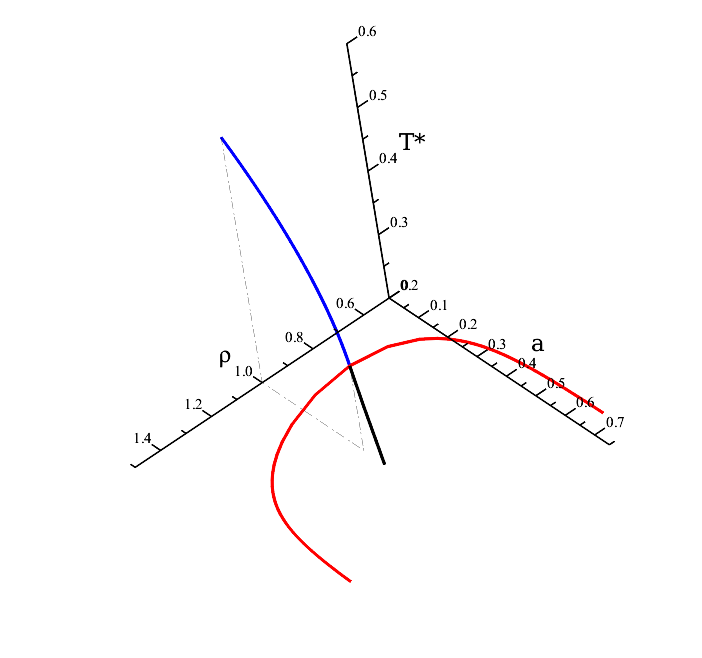
\includegraphics[width=0.6\textwidth]{img/T-rho-a-phase-diagram4.png}
		\includegraphics[width=0.5\textwidth]{img/fig1_v2.pdf}
		\caption{Phase diagram of the double-occupancy cell model of a fluid with Curie-Weiss interaction for the system of distinguishable particles. Blue line: the line of critical points at $a \leq a_{\rm tc}$. Red lines: the lines of critical points at $a > a_{\rm tc}$. Black line: the line of triple points, which exists in the interval $a_{\rm tp} < a < 0.5$. All the line meet at the tricritical point.}
		\label{fig:T-rho-a-3d}
	\end{figure}
	
	Note that in the region where two critical points exist, the sum of two critical densities always remains the same
	\begin{equation}
		\rho^{*(1)}_c + \rho^{*(2)}_c = 2.
	\end{equation}
	
	\subsection{Coexistence curves}\label{sec:coex}
	Having found critical point coordinates for different values of $a$, we are now proceeding with building the coexistence curves. Based on the analysis of Section~\ref{sec:cp}, we present phase diagrams for the double-occupancy cell model with the Curie-Weiss interaction for a set of selected increasing values of $a$, namely $a=0.3,$ $0.375,$ $0.45,$ and $0.6$, see Fig.~\ref{fig:phase_diagrams}.
	
	\begin{figure}
		\centering
		\begin{subfigure}[b]{0.23\textwidth}
			\centering
			%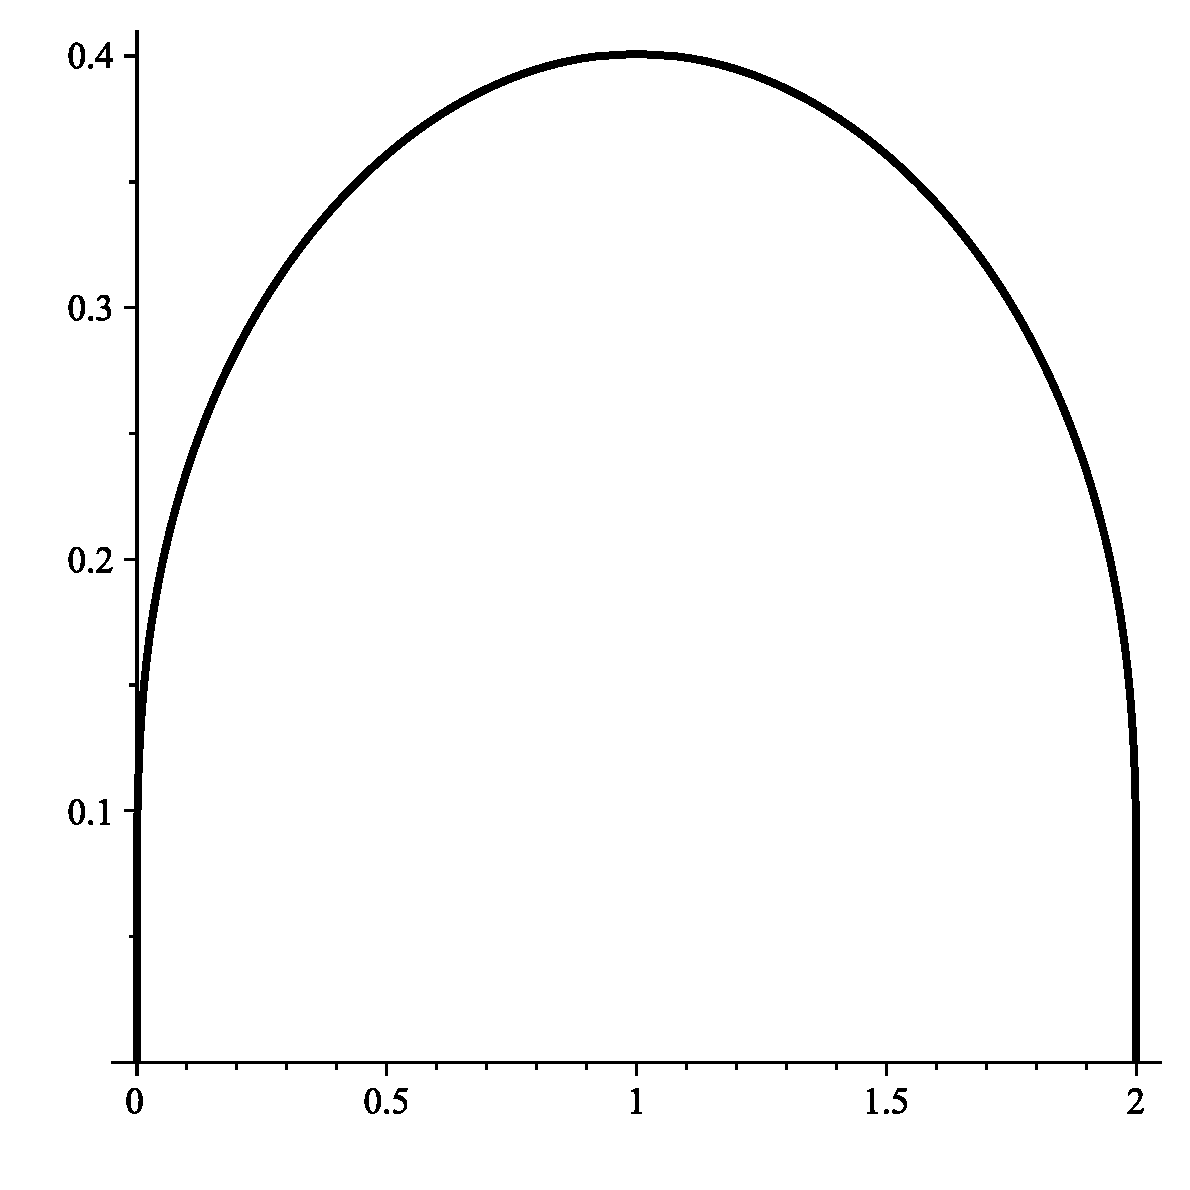
\includegraphics[width=\textwidth]{img/coex_a_03}
			\includegraphics[width=\textwidth]{img/fig2a.pdf}
			\caption{$a=0.3$}
			\label{fig:pd1}
		\end{subfigure}
		\hfill
		\begin{subfigure}[b]{0.23\textwidth}
			\centering
			%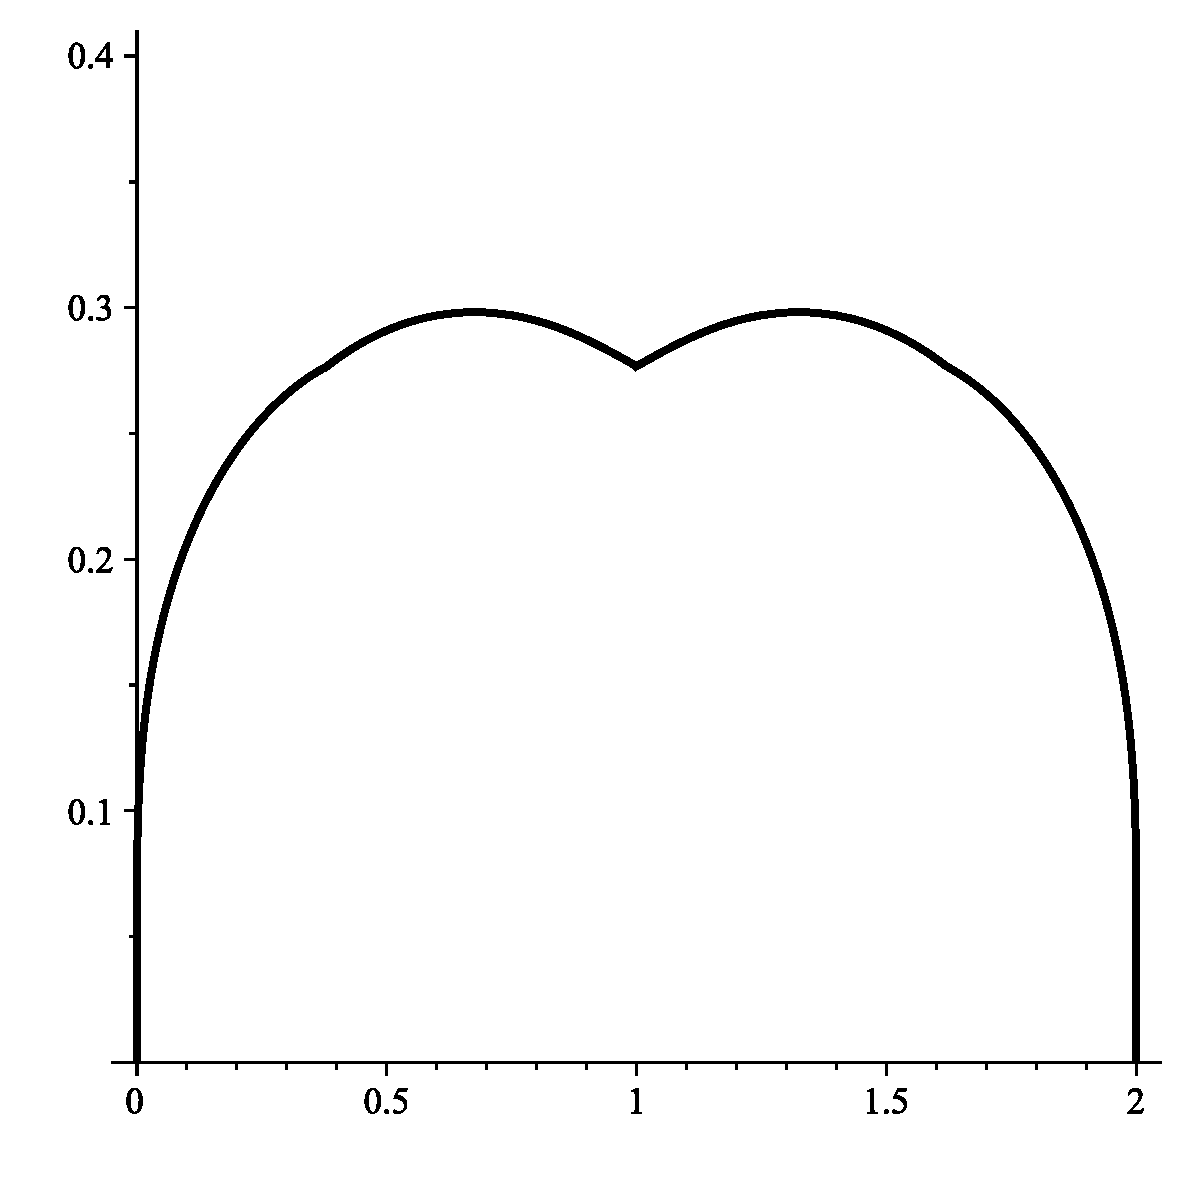
\includegraphics[width=\textwidth]{img/coex_a_0375_a}
			\includegraphics[width=\textwidth]{img/fig2b.pdf}
			\caption{$a=0.375$}
			\label{fig:pd2}
		\end{subfigure}
		\hfill
		\begin{subfigure}[b]{0.23\textwidth}
			\centering
			%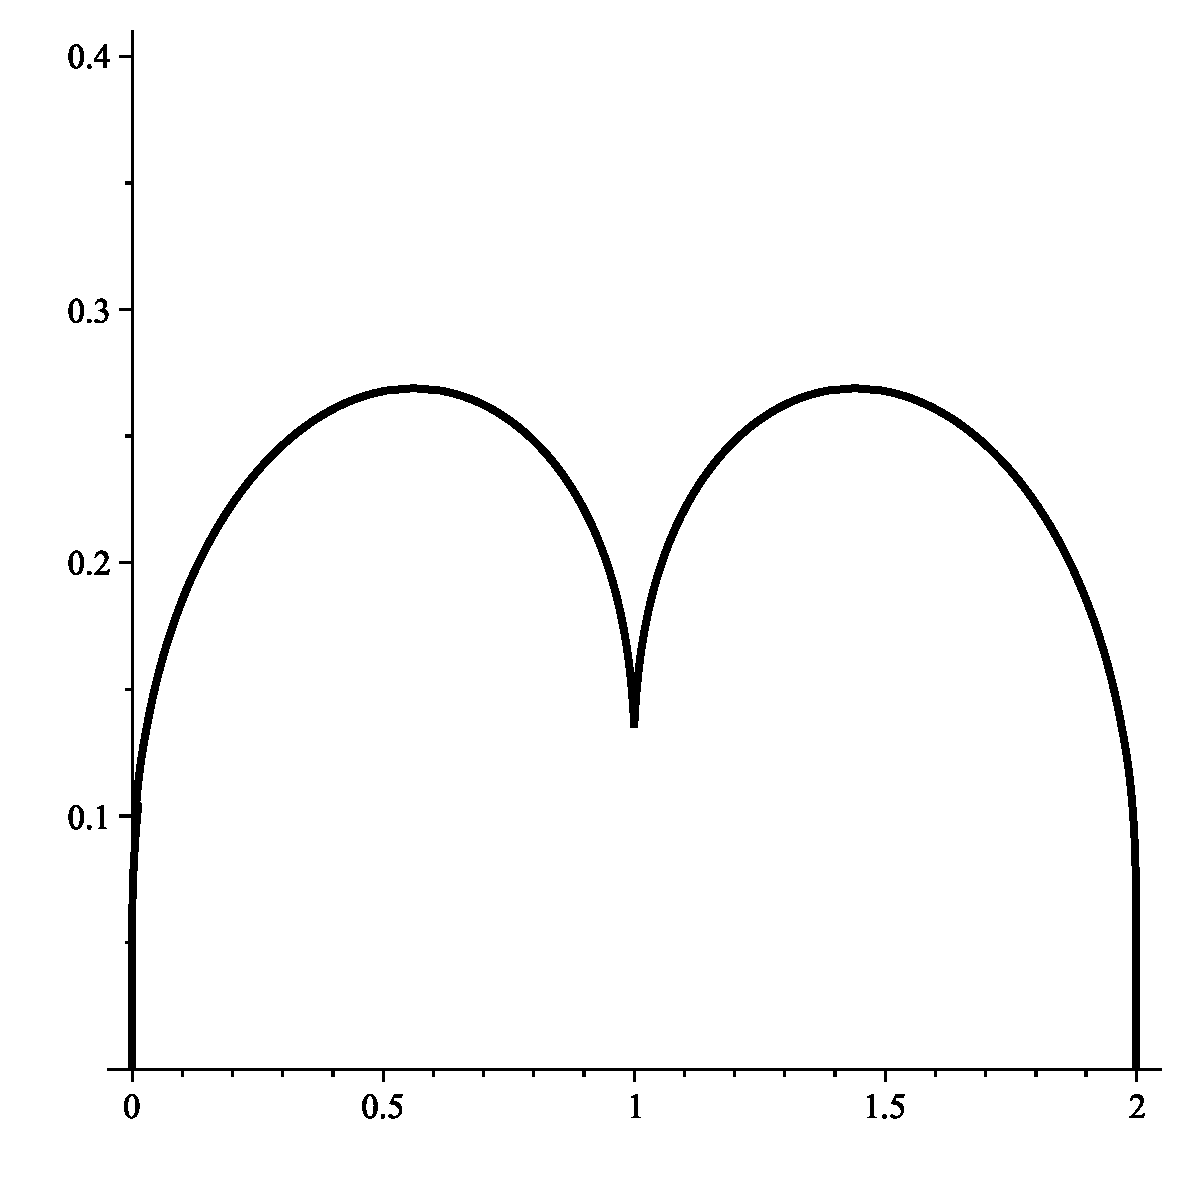
\includegraphics[width=\textwidth]{img/coex_a_045_a}
			\includegraphics[width=\textwidth]{img/fig2c.pdf}
			\caption{$a=0.45$}
			\label{fig:pd3}
		\end{subfigure}
		\hfill
		\begin{subfigure}[b]{0.23\textwidth}
			\centering
			%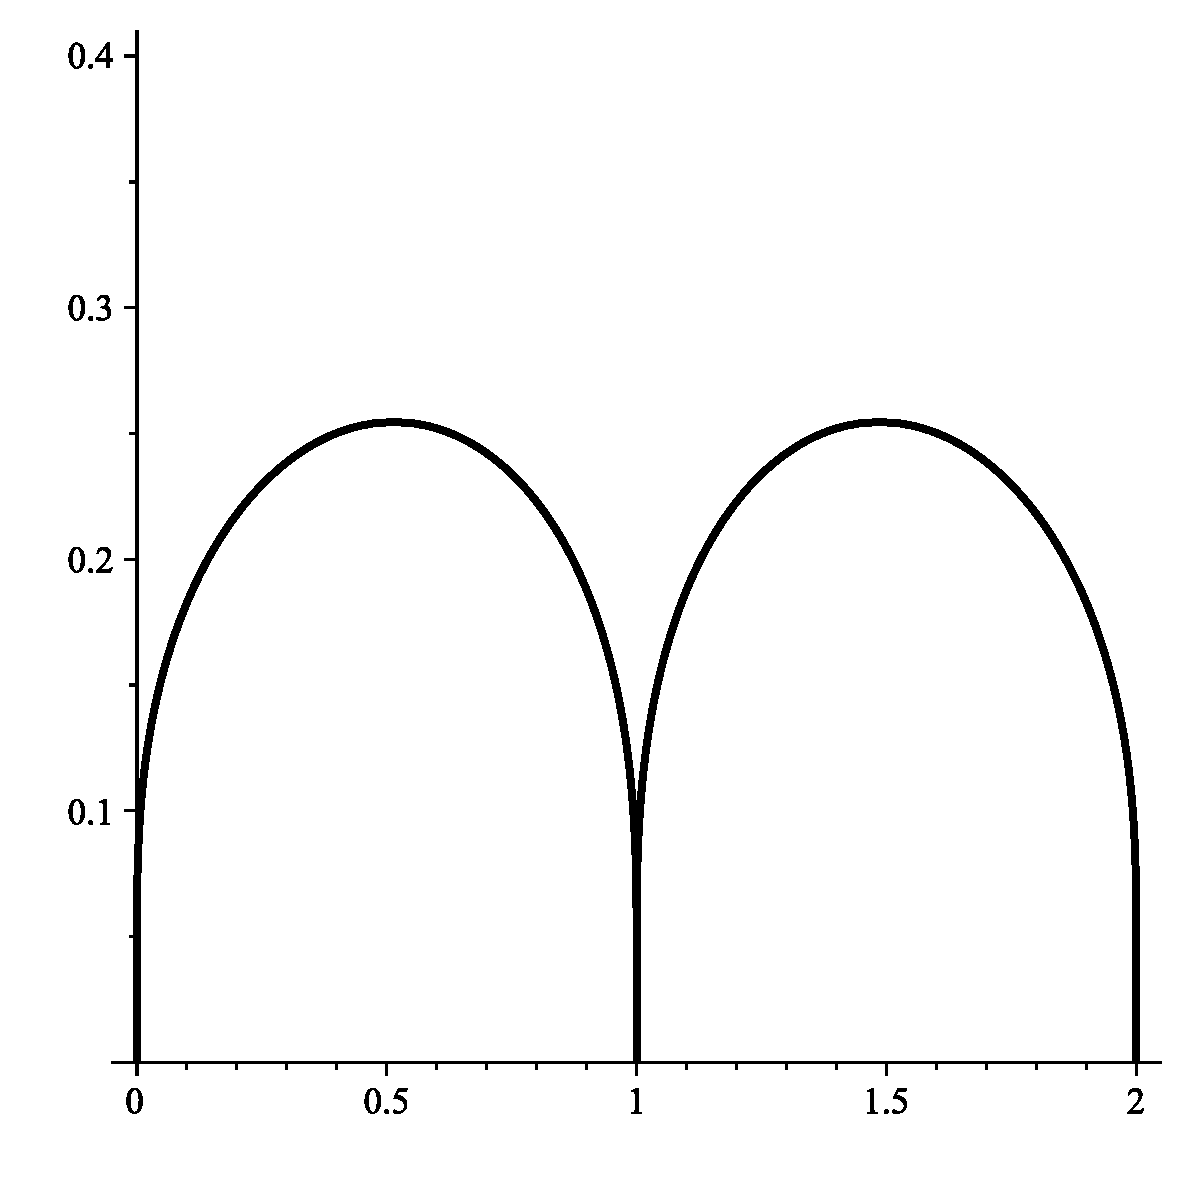
\includegraphics[width=\textwidth]{img/coex_a_06_a}
			\includegraphics[width=\textwidth]{img/fig2d.pdf}
			\caption{$a=0.6$}
			\label{fig:pd4}
		\end{subfigure}
		
		\caption{The $T^* - \rho^*$ phase diagrams of the double-occupancy lattice gas for the case of distinguishable particles at different values of $a=\Delta/J$. Solid lines are the coexistence curves. {\bf (a)}: The coexistence curve between phases I and III ends at the critical point. {\bf (b)} and {\bf (c)}: The coexistence curves between phases I and II, as well as between II and III are present in the temperature interval $T^*_{\rm tr} \leq T^* \leq T^*_c$, each ending at its own critical point. For $T^* \leq T^*_{\rm tr}$, phases I and III coexist. $T^*_{\rm tr}$ is the temperature of the triple point. {\bf (d)}: The coexistence curves between phases I and II, as well as between II and III are present for $0 \leq T^* \leq T^*_c$, each ending at its own critical point.}
		\label{fig:phase_diagrams}
		
	\end{figure}
	
	When the ratio of repulsion to attraction couplings is small enough, the coexistence line of the double occupancy cell model resembles that of a single-occupancy lattice gas. In particular, there is one critical point, and for temperatures below the critical value, a symmetric coexistence curve between two phases exists. The two phases are characterized by low and high densities. Figure~\ref{fig:pd1} shows the phase diagram in the $T^* - \rho^*$ plane, which is a typical diagram for small values of $a$, specifically for $a \leq a_{\rm tc}$, where $a_{\rm tc} = \frac{1}{2}\ln 2$ in the case of distinguishable particles. At $a=0.3$, the coordinates of the critical point are $T^*_c = 0.401$, $\rho^*_c=1.0$, and $P^*_c=0.144$. 
	
	As soon as $a$ becomes greater than $\frac{1}{2}\ln 2$, the line of critical points bifurcates, and two critical points appear. Figure~\ref{fig:pd2} illustrates the phase diagram at $a=0.375$. Two critical points are observed with the same critical temperature $T^*_c = 0.298$, but with different densities, $\rho^{*(1)}_c = 0.676$ and $\rho^{*(2)}_c=1.32$, and different pressures, $P^{*(1)}_c=0.073$ and $P^{*(1)}_c=0.086$. Now, between the low density phase (let us call it phase I) and the high density phase (let us call it phase III), a phase of intermediate density appears (let us call it phase II). But the phase II exists only for temperatures down to some temperature $T^*_{\rm tr}$. Below that temperature, the phase transition occurs directly between phase I and phase III. The point $(T^*_{\rm tr}, P^*_{\rm tr})$ is called \textit{the triple point}, since this is the point where three phases, namely phase I, phase II, and phase III, can coexist at the same pressure and temperature, but at different values of densities.
	
	As the value of $a$ is increased even more, the phase diagram changes in such a way that the difference between the critical densities increases, the critical temperature slowly decreases, and the temperature of the triple-point temperature decreases quite notably. The phase diagram at $a=0.45$ is demonstrated in Fig.~\ref{fig:pd3}. 
	
	At some value of $a$, namely at $a \approx 0.5$, the triple point temperature becomes zero, and for greater $a$ the triple point does not exist anymore, as is seen in Fig.~\ref{fig:pd4} where the phase diagram is presented for $a=0.6$. For such high values of $a$, there are three phases at sufficiently low temperatures. At very low temperatures, e.g. $T^* < 0.05$, the phase densities are $\rho^*_{I} \approx 0$, $\rho^*_{II} \approx 1$, and $\rho^*_{III} \approx 2$, and remain nearly constant. This means that we observe pronounced phase transitions between three phases of integer-valued densities.
	
	Figure~\ref{fig:combined}  combines the results presented in Figs.~\ref{fig:T-rho-a-3d} and~\ref{fig:phase_diagrams}. The coexistence curves are presented in the three dimensional space along with the critical point lines and the triple-point line.
	
	\begin{figure}
		\centering
		%\includegraphics[width=0.6\textwidth]{img/full3d_2_edited_1.pdf}
		%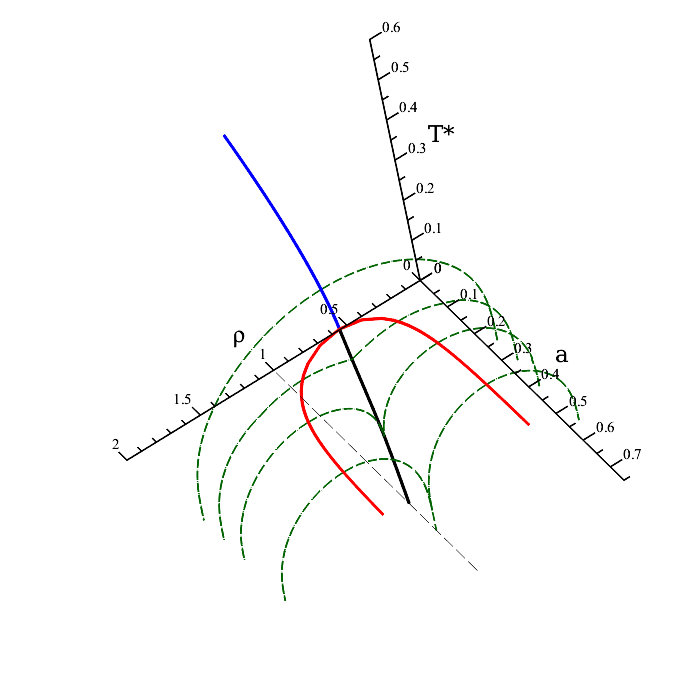
\includegraphics[width=0.6\textwidth]{img/3Dcombo-3.png}
		\includegraphics[width=0.5\textwidth]{img/fig3_v3.pdf}
		\caption{The phase diagram in the $(T^*,\rho^*,a)$-space for the case of distinguishable particles. This figure combines results of Figs.~\ref{fig:T-rho-a-3d} and~\ref{fig:phase_diagrams} in one view. Green dashed lines: the coexistence curves at several values of parameter $a$: $a=0.3$, $a=0.375$, $a=0.45$, and $a=0.6$. Blue and Red lines are the locus of critical points. Black line is the line of triple points.}
		\label{fig:combined}
	\end{figure}
	
	\subsection{Triple point coordinates}
	In the interval $\frac{1}{2}\ln 2 < a < 0.5$, the system possesses a triple point, where three phases -- phase I, phase II, and phase III -- characterized by different densities, can coexist at the same temperature and pressure. The numerical results for the triple-point coordinates are presented in Table~\ref{tab:triple-line} at some values of $a$ in the considered interval.
	
	\begin{table}[h]
		\centering
		\caption{Triple point coordinates of the double-occupancy cell model for the case of distinguishable particles. A triple point exists in the system in the interval $a_{\rm tc} \leq \Delta/J < 0.5$, where $a_{\rm tc} = \frac{1}{2} \ln 2$.}
		\begin{tabular}{c|c|c|c|c|c}
			\toprule
			$a=\Delta/J$ & $T^*_{\rm tr}$ & $P^*_{\rm tr}$ & $\rho^{*(I)}_{\rm tr}$ & $\rho^{*(II)}_{\rm tr}$ & $\rho^{*(III)}_{\rm tr}$ \\
			\midrule
			0.500 & $\approx 0.0$ & $\approx 0.0$ & $\approx 0.0$ & 1.0 & $\approx 2.0$ \\
			0.475 & 0.0719370 & $6.93 \cdot 10^{-5}$ & $9.69 \cdot 10^{-4}$  & 1.0 & 1.99903 \\
			0.450 & 0.135275 & $3.585 \cdot 10^{-3}$ & 0.0292224 & 1.0 & 1.97078 \\
			0.425 & 0.185875 & 0.0143790 & 0.0981956 & 1.0 & 1.90180 \\
			0.400 & 0.231382 & 0.0320139 & 0.207212 & 1.0 & 1.79279 \\
			0.375 & 0.276725 & 0.0569574 & 0.380556 & 1.0 & 1.61944 \\
			0.350 & 0.325987 & 0.0915080 & 0.766700 & 1.0 & 1.23330 \\
			$\frac{1}{2}\ln 2 \approx 0.346574$ & $0.333333 = \frac{1}{3}$ & 0.0972532 & 1.0 & 1.0 & 1.0 \\
			\bottomrule
		\end{tabular}
		\label{tab:triple-line}
	\end{table}
	
	It is worth noting that in the classical, single-occupancy lattice gas models the triple point does not exist, since there are only two phases in the model. In contrast, multiple-occupancy models may possess one or more triple points. When we originally studied the multiple-occupancy cell model of a fluid~\cite{KKD20, KD22}, the triple points were not observed. In~\cite{KDPRS26}, we managed to obtain the triple point with the help of introducing state-dependent interactions. In particular, the pair interaction between particles was assumed to depend on temperature, and this assumption led to the emergence of a triple point~\cite{KDPRS26}. In the multiple-occupancy cell model with unrestricted occupancy, there is a strict limitation $a \geq 1$, thus we could not consider the region $a < 1$. In the double-occupancy model, this restriction is not required, and the triple points naturally emerge in the system in the interval $a_{\rm tc} < a < 1.0$.
	
	\subsection{Limiting cases}
	When comparing our results for some limiting cases from Table~\ref{tab:critical-points} and Table~\ref{tab:triple-line} with the results of Ref.~\cite{HKBHK25}, we may notice the following discrepancies. The first one is that at $\Delta = 0$, the critical temperature for the cell model is $T^*_c=0.586$, while for the Blume-Capel model it was found to be $T^*_c=3/2$. The second one is that at the tricritical point, $a_{\rm tc}=\frac{1}{2}\ln 2.0$ for the cell model, and $a_{\rm tc}=\frac{2}{3} \ln 2$ for the Blume-Capel model. We conclude that this discrepancies are associated with the fact that in this Section we considered distinguishable particles and the grand partition function contained multipliers of type $\frac{1}{n_l!}$. Let us now proceed with consideration of the cell model for a system of indistinguishable particles.
	
	\section{Indistinguishable particles} \label{sec:indist}
	In this Section, we consider the cell model for a system of indistinguishable particles characterized by the grand partition function~\eqref{Xi:indist}. The method of calculation is the same as presented in Section~\ref{sec:distinct}, and the analytical results of Eqs.~\eqref{eq:Xi_z} -- \eqref{eq:rho} remain the same if we account for the changed form for the special functions $K_0$ and $K_j$:
		\begin{equation}
		\label{def:K0ind}
		K_0(T^*;z) = \sum_{n=0}^{2} \left(T^{*3/2}\right)^n \exp\left(zn - \frac{a}{T^*}n^2\right),
	\end{equation}
	\begin{equation}
		K_j(T^*; z) = \sum_{n=0}^2 n^j \left(T^{*3/2}\right)^n \exp\left(z n - \frac{a}{T^*}n^2\right),
	\end{equation}
	where the multiplier $1/n!$ is missing compared to Eqs~\eqref{def:K0} and~\eqref{def:Kj}.
	
	\begin{table}[h]
	\centering
	\caption{Critical point coordinates of the double-occupancy cell model for the case of indistinguishable particles. At the tricritical point, $a_{\rm tc} = \frac{2}{3} \ln 2$. For any value $a \leq a_{\rm tc}$, there is a single critical point; for any value $a > a_{\rm tc}$, there are two critical points.}
		\begin{tabular}{c|c|c|c|c|c}
			\toprule
			$a=\Delta/J$ & $T^*_c$ & $\rho^{*(1)}_c $ & $P^{*(1)}_c$ & $\rho^{*(2)}_c$ & $P^{*(2)}_c$\\
			\midrule
			5.0 & $0.25 = \frac{1}{4}$ & $0.5 = \frac{1}{2}$ & $0.0482868 \approx \frac{1}{4}\left(\ln 2 - \frac{1}{2}\right)$ & $1.5 = \frac{3}{2}$ & 9.04829 \\
			2.0 & 0.250000 & 0.500000 & 0.0482868 & 1.50000 & 3.04829 \\
			1.5 & 0.250006 & 0.500018 & 0.0482895 & 1.49998 & 2.04830 \\
			1.2 & 0.250068 & 0.500204 & 0.0483169 & 1.49980 & 1.44842 \\
			1.0 & 0.250340 & 0.501020 & 0.0484374 & 1.49898 & 1.04895 \\
			0.9 & 0.250766 & 0.502302 & 0.0486268 & 1.49770 & 0.849771 \\
			0.8 & 0.251749 & 0.505276 & 0.0490662 & 1.49472 & 0.651669 \\
			0.7 & 0.254116 & 0.512503 & 0.0501341 & 1.48750 & 0.456193 \\
			0.6 & 0.260379  & 0.532171 & 0.0530373 & 1.46783 & 0.267878 \\
			0.5 & 0.283117 & 0.611865 & 0.0645817 & 1.38814 & 0.106814 \\
			$\frac{2}{3}\ln 2 \approx 0.462098$ & $\frac{1}{3} \approx 0.333333$ & 1.00000 & 0.0972532 & 1.00000 & 0.0972532\\
			0.45 & 0.378647 & 1.0 & 0.130182 & - & - \\
			0.4 & 0.452377 & 1.0 & 0.172407 & - & - \\
			0.3 & 0.532359 & 1.0 & 0.204622 & - & - \\
			0.2 & 0.587241 & 1.0 & 0.219645 & - & - \\
			0.1 & 0.630545 & 1.0 & 0.227849 & - & - \\
			0.0 & $\frac{2}{3} \approx 0.666667$  & 1.0 & $0.232408 \approx \frac{2}{3} \ln 3 - \frac{1}{2}$  & - & - \\
			\bottomrule
		\end{tabular}
		\label{tab:critical-points-ind}
	\end{table}
	
	\begin{table}[h]
	\centering
	\caption{Triple point coordinates of the double-occupancy cell model for the case of indistinguishable particles. A triple point exists in the system in the interval $a_{\rm tc} \leq \Delta/J < 0.5$, where $a_{\rm tc} = \frac{2}{3} \ln 2$.}
		\begin{tabular}{c|c|c|c|c|c}
			\toprule
			$a=\Delta/J$ & $T^*_{\rm tr}$ & $P^*_{\rm tr}$ & $\rho^{*(I)}_{\rm tr}$ & $\rho^{*(II)}_{\rm tr}$ & $\rho^{*(III)}_{\rm tr}$ \\
			\midrule
			0.500 & $\approx 0.0$ & $\approx 0.0$ & $\approx 0.0$ & 1.0 & $\approx 2.0$ \\
			0.495 & 0.151204 & $6.03783 \times 10^{-3}$ & 0.0457859 & 1.0 & 1.95421 \\
			0.490 & 0.182706 & 0.0134364 & 0.0924053 & 1.0 & 1.90759 \\
			0.485 & 0.208422 & 0.0221600 & 0.145810 & 1.0 & 1.85419 \\
			0.480 & 0.232284 & 0.0324399 & 0.209923 & 1.0 & 1.79008 \\
			0.475 & 0.256113 & 0.0447467 & 0.291335  & 1.0 & 1.70867 \\
			0.470 & 0.281540 & 0.0600103 & 0.404731 & 1.0 & 1.59527 \\
			0.465 & 0.311272 & 0.0804435 & 0.600782 & 1.0 & 1.39922 \\
			$\frac{2}{3}\ln 2 \approx 0.462098$ & $0.333333 = \frac{1}{3}$ & 0.0972532 & 1.0 & 1.0 & 1.0 \\
			\bottomrule
		\end{tabular}
		\label{tab:triple-line-ind}
	\end{table}
	
	Qualitatively, the behavior of the model and its phase diagram described in~Sections~\ref{sec:cp}--\ref{sec:coex} remains the same.
	However, the numerical results change for the coordinates of the critical and triple points. The corresponding values for the case of indistinguishable particles are presented in Tables~\ref{tab:critical-points-ind} and~\ref{tab:triple-line-ind}. In particular, we can see that at $\Delta = 0$, the critical temperature $T^*_c = \frac{2}{3}$, which coincides with the value for the Blume-Capel model~\cite{HKBHK25}. The tricritical point is located at $(T^*_{\rm tc} = \frac{1}{3}; a_{\rm tc} = \frac{2}{3} \ln 2)$, which is the same as in the Blume-Capel model~\cite{HKBHK25} as well. This leads us to the conclusion that for the proper isomorphism between a cell model (lattice gas) and the Blume-Capel model, the system of indistinguishable particles must be considered.
	
	Note that the interval where the triple point exists is shorter for the case of indistinguishable particles. It is $\frac{2}{3}\ln 2 < a < 0.5$ compared to $\frac{1}{2} \ln 2 < a < 0.5$ for the case of distinguishable particles.
	
	
	\section{Different phases and their interpretation}
	For sufficiently large values of $a$ and sufficiently low temperatures, the double-occupancy cell model exhibits three distinct equilibrium phases. Following our previous works~\cite{KD22}, we denote them by phase I, phase II, and phase III in the order of increasing density. At very low temperatures, these phases are characterized approximately by the densities $\rho^{*}_{\rm I} \approx 0.0$, $\rho^*_{\rm II} \approx 1.0$, and $\rho^*_{\rm III} \approx 2.0$, respectively. The phase transitions between them are first-order and terminated at critical points, giving rise to the phase diagrams discussed in Section~\ref{sec:distinct}.
	
	Since the phases differ primarily by their densities, alternative terminology can also be adopted. In studies of fluids exhibiting two critical points, it is common to refer to the corresponding phases as a gas, a low-density liquid (LDL), and a high-density liquid (HDL)~\cite{Franzese07}. In the present work, this terminology is used only as a density-based classification and does not imply any structural distinction between the phases, since the mean-field model considered here does not explicitly account for local ordering. Within this interpretation, phase I corresponds to the gas phase, while phases II and III represent two liquid states of different densities. The coexistence line between phases II and III then corresponds to a liquid-liquid phase transition, terminating at a liquid-liquid critical point.
	
	A different terminology was used in~\cite{LYZ21}, where analogous phases were referred to as gas, liquid, and crystal states. In the present work, however, we avoid the term ``crystal'', since the Curie-Weiss version of the model considered here does not explicitly describe translational ordering. Instead, the high-density phase is more naturally interpreted as a dense fluid phase. This viewpoint is further supported by the behavior of the pair distribution function discussed in Appendix~\ref{sec:pair}, which resembles that of a high-density mean-field fluid~\cite{LBH00} rather than a crystalline solid.
	
	The existence of three fluid phases separated by first-order transition lines is a known feature of systems with soft-core interactions. In particular, models with attractive soft-core potentials were shown to exhibit gas, low-density liquid, and high-density liquid phases, together with two critical points~\cite{Franzese07}. Similar phenomenology has been reported experimentally for several materials, including liquid phosphorus~\cite{KMUetal00,MFCM03,YKP21} and triphenyl phosphite~\cite{KT04}. Additional examples can be found in the review sections in Refs.~\cite{dONCB06,Franzese07}. Therefore, despite its simplicity, the double-occupancy cell model reproduces the essential thermodynamic features associated with fluid-fluid and liquid-liquid phase transitions in systems possessing multiple density states.
	
	\section{Conclusions}
	We have studied a double-occupancy cell model of a fluid with Curie-Weiss interaction, in which each cell can contain at most two particles. The interaction consists of a global attractive contribution acting between all particle pairs and a local repulsive contribution when two particles occupy the same cell. We have shown that this model is isomorphic to the Blume-Capel model on a complete graph through a simple transformation from spin variables  $\sigma_l \in \{-1, 0, +1\}$ to occupancy variables $n_l \in \{0, 1, 2\}$. Using the grand-canonical formalism previously developed for multiple-occupancy cell models, we obtained a description of the thermodynamic properties and phase behavior of the system.
	
	Depending on the ratio between the repulsive and attractive couplings, the model exhibits several qualitatively distinct thermodynamic regimes. In particular, we identified regions of the phase diagram containing a single critical point, two critical points, a tricritical point, and a triple point. For sufficiently strong repulsion, three fluid phases of different densities coexist in the system, giving rise to two first-order phase-transition lines, each terminating at its own critical point. The coexistence between the intermediate-density and high-density phases may be interpreted as a liquid-liquid phase transition terminating at a liquid-liquid critical point. These results demonstrate that a remarkably rich phase behavior can emerge already in a model with the simple occupancy restriction $n_l \le 2$.
	
	We considered both distinguishable and indistinguishable particles. While the phase behavior is qualitatively similar in the two cases, the formulation for indistinguishable particles reproduces the known limiting results for the Blume-Capel model on a complete graph, including the location of the tricritical point. This provides an additional confirmation of the isomorphism between the two models and indicates that the indistinguishable-particle formulation is the natural lattice-gas counterpart of the Blume-Capel model.
	
	The present model is of interest from several perspectives. As a lattice-gas model, it provides a simple analytically tractable framework for studying phase transitions in systems with multiple cell occupancy. From the viewpoint of soft-matter physics, it represents a minimal mean-field description of particles interacting through a competition between bounded local repulsion and long-range attraction. More broadly, the model demonstrates that the interplay between these two ingredients alone is sufficient to generate gas-liquid and liquid-liquid coexistence, two critical points, and triple points. It therefore provides a mean-field realization of a fluid exhibiting both gas-liquid and liquid-liquid phase transitions while remaining directly connected to the well-known Blume-Capel model.

	
	\bmhead{Acknowledgements} This work was supported by the National Research Foundation of Ukraine under the project No. 2023.03/0201. The authors are
	deeply grateful to all warriors of the Ukrainian Armed Forces, living and fallen, for making this research possible
	
	%\pagebreak
	\appendix
	
	\section{Pair distribution function}\label{sec:pair}
	In this Appendix, we present the results for the pair distribution function $g^{(2)}$ of the double-occupancy cell model. The details of calculations can be found in~\cite{RDKPS25arxiv3}, where this quantity was obtained for the multiple-occupancy cell model. The final expression for $g^{(2)}$ as an explicit function of $T^*$ and an implicit function of $\mu^*$ is 
	\begin{equation}
		\label{eq:g2_in_z}
		g^{(2)} = \frac{\left[{K}_2(T^*; \bar{z}_{\rm max}) - {K}_1(T^*; \bar{z}_{\rm max})\right] {K}_0(T^*; \bar{z}_{\rm max})}{{K}_1(T^*; \bar{z}_{\rm max})^2}.
	\end{equation}
	
	The spatial dependency of the pair distribution function is expressed as
	\begin{equation}
		\label{g2_r}
		g^{(2)}({\vb r}_1, {\vb r}_2) =  \left\{
		\begin{array}{ll}
			1, & \text{if } \nexists \Delta_l ({\vb r}_1, {\vb r}_2 \in \Delta_l),
			\\
			\frac{\langle n(n-1) \rangle_{Q}}{\langle n \rangle_{Q}^2}, & \text{if } \exists \Delta_l ({\vb r}_1, {\vb r}_2 \in \Delta_l),
		\end{array}
		\right.
	\end{equation}
	where
	\begin{equation}
		\langle n \rangle_{Q} = \rho^*,
	\end{equation}
	\begin{equation}
		\langle n(n-1) \rangle_{Q} = \sum_{n=0}^{2} n(n-1) Q_{T^*, \mu^*}(n) = 2 Q_{T^*, \mu^*}(2),
	\end{equation}
	and the probability measure $Q_{T^*,\mu^*}(n)$~\cite{KKD20} is given by:	
	\begin{equation*}
		Q_{T^*,\mu^*}(n) = \frac{\left(T^{*3/2}\right)^n}{K_0(T^*; \bar{z}_{\rm max}) n!} \exp\left(\bar{z}_{\rm max}n - \frac{a}{T^*}n^2 \right),
		\quad n \in \{0,1,2\},
	\end{equation*}
	in the case of distinguishable particles, and by
	\begin{equation*}
		Q_{T^*,\mu^*}(n) = \frac{\left(T^{*3/2}\right)^n}{K_0(T^*; \bar{z}_{\rm max})} \exp\left(\bar{z}_{\rm max}n - \frac{a}{T^*}n^2 \right),
		\quad n \in \{0,1,2\},
	\end{equation*}
	in the case of indistinguishable particles.
	
	\begin{figure}[htbp]
		\centering
		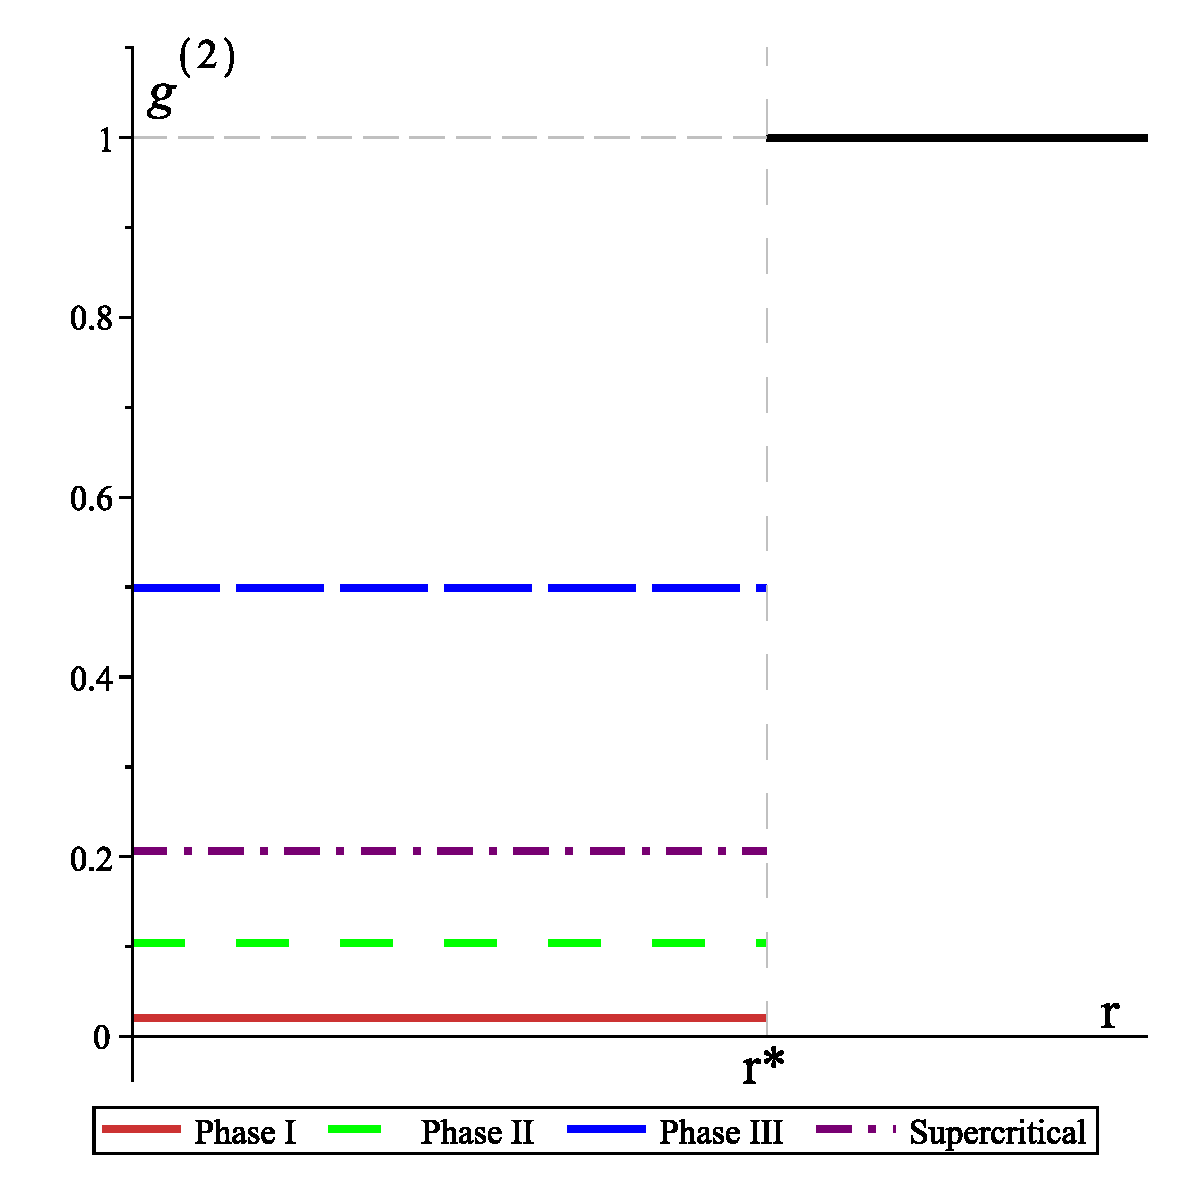
\includegraphics[width=0.5\textwidth]{img/g2_vs_r}
		\caption{\label{fig:g2_r} Pair distribution function $g^{(2)}({\vb r}_1, {\vb r}_2)$ as a function of separation $r = \abs{{\vb r}_1 - {\vb r}_2}$. The quantity $r^*$ denotes distance from the point with coordinate ${\vb r}_1$ to the boundary of the cubic cell containing ${\vb r}_1$, in the direction of ${\vb r}_2$. The results are presented for the system of distinguishable particles, at $a=0.5$. Phase I: $T^* = 0.25$, $\rho^*=0.1$; Phase II: $T^* = 0.2$, $\rho^* = 0.5$; Phase III: $T^*_c = 0.25$, $\rho^* = 1.9$; Supercritical: $T^* = 0.5$, $\rho^* = 0.5$. At $r > r^*$, $g^{(2)} = 1$.}
	\end{figure}
	
	In Fig.~\ref{fig:g2_r}, the spatial dependency of $g^{(2)} (\vb{r}_1, \vb{r}_2)$, Eq.~\eqref{g2_r}, is illustrated for the system of distinguishable particles at $a=0.5$ and the following selected states: for phase I, $T^*=0.25$ and $\rho^*=0.1$; for phase II, $T^*=0.2$ and $\rho^*=1.0$; for phase III, $T^*=0.25$ and $\rho^*=1.9$; and for supercritical state, $T^*=0.5$ and $\rho^*=0.5$. As is seen from the plot, $g^{(2)}$ at any selected $T^*$ and $\rho^*$ is presented as a step function. While $\vb{r}_1$ and $\vb{r}_2$ are located within one cell, $g^{(2)}$ takes on a value that is dependent on temperature and density. However, as soon as the coordinates of two particles belong to different cells, the pair distribution function becomes unity. At high densities, this is known as high-density mean field fluid, the behavior which is also observed in systems with soft interactions~\cite{LBH00}. Therefore, the result of this Appendix supports the interpretation of phase III as a dense fluid rather than a crystal.	

	
	
	
	%%===========================================================================================%%
	%% If you are submitting to one of the Nature Portfolio journals, using the eJP submission   %%
	%% system, please include the references within the manuscript file itself. You may do this  %%
	%% by copying the reference list from your .bbl file, paste it into the main manuscript .tex %%
	%% file, and delete the associated \verb+\bibliography+ commands.                            %%
	%%===========================================================================================%%
	
	%\pagebreak
	
	\bibliography{articles,books}
	%\bibliography{sn-bibliography}% common bib file
	%% if required, the content of .bbl file can be included here once bbl is generated
	%%\input sn-article.bbl
	
\end{document}

\section{Drafts and ideas}
The reconsideration of the Blume-Capel model from the lattice gas / cell fluid perspective is valuable in itself. It gives an opportunity to look at the familiar model from a different perspective.

Regarding the isomorphism between the cell fluid model and the Blume-Capel spin model, we conclude that the system of indistinguishable particles must be considered.

The case of indistinguishable particles is isomorphic to the Blume-Capel model much better.


The line of triple points can be also interpreted as the line of first order phase transition between phase I and phase III.

The critical temperature becomes slower as the on-site interaction becomes stronger.

\section{Refs.}
Consider Refs. \cite{PCMR19}, \cite{VT25}, \cite{BB04}, \cite{SBFMS04}, \cite{Franzese07}, \cite{VF10}

In \cite{dOT19}, two critical points are observed in phospholipid monolayers.

Attempts to map Blume-Capel to lattice gas were made in~\cite{LS75}, ~\cite{BB01}, ~\cite{LDZ21} but it was mapped to multi-component lattice gas, rather than to multiple-occupancy.



